%----------------------------------------------------------------------------------------
%	PACKAGES AND THEMES
%----------------------------------------------------------------------------------------
\documentclass[aspectratio=169,xcolor=dvipsnames]{beamer}
\usetheme{Simple}
\usepackage{amsfonts, amssymb, amsmath}
\usepackage{caption}
\usepackage{subcaption}
\usepackage{hyperref}
\usepackage{pdfpages}
\usepackage[backend=biber, sorting=none]{biblatex}
\addbibresource{main.bib}
\AtBeginBibliography{\small}
\usepackage{graphicx} % Allows including images
\usepackage{booktabs} % Allows the use of \toprule, \midrule and \bottomrule in tables
\renewcommand{\inserttotalframenumber}{\pageref{lastslide}}

%----------------------------------------------------------------------------------------
%	TITLE PAGE
%----------------------------------------------------------------------------------------

% The title
\title[short title]{Posture Detection}
\subtitle{Monitor Posture in Real-time using Gyroscope.}
\vspace{10cm}
\author[Pin-Yen]{Pratyusha R - C Ramprakash - Skanda Prasad}
\institute % Your institution may be shorthand to save space
{
    % Your institution for the title page
    Department of Electronics and Communication Engineering

    6th Semester, A Section 
    \vskip 3pt
}
\date{June 24, 2021} % Date, can be changed to a custom date


%----------------------------------------------------------------------------------------
%	PRESENTATION SLIDES
%----------------------------------------------------------------------------------------

\begin{document}

\begin{frame}
    % Print the title page as the first slide
    \begin{figure}
     \centering
     \begin{subfigure}[b]{0.49\textwidth}
         \centering
         \includegraphics[scale=0.35]{drpt.PNG}
     \end{subfigure}
     \hfill
     \begin{subfigure}[b]{0.49\textwidth}
         \centering
         \includegraphics[scale=0.35]{New_NIE_Logo.png}
     \end{subfigure}
     \end{figure}
    \titlepage
\end{frame}
%---------------------------------------------------

\begin{frame}{Overview}
    \tableofcontents
\end{frame}

%------------------------------------------------
\section{Introduction.}
%------------------------------------------------

\begin{frame}{Introduction}
        \vspace{0.5cm}
        \begin{itemize}
        \item Bad habits such as slouching cause muscle fatigue and tension that ultimately lead to poor posture.
        \item Slouching can cause the spinal ligaments to stretch beyond their healthy limit, and poor posture can strain your spinal discs. 
        \item To correct bad posture it is crucial to monitor posture. 
        \item \textit{" If you can’t measure it, you can’t improve it."} –\textit{ Peter Drucker}
    \end{itemize}
    \hfill
     \begin{figure}
        \centering
        \includegraphics[scale=0.25]{slouching-bad-computer-posture.jpg}        
        \caption{"Depicting Slouching Posture"}
        \label{fig:good}
    \end{figure}
\end{frame}

%------------------------------------------------




%------------------------------------------------
\section{Data Collection}



%-----------------------------------------------------------

% \begin{frame}{Proposed Solution}

        
%         \begin{enumerate}
%         \item Collect Gyroscope data with Arduino or Esp8266.
%         \item 
%         \item The python scripts sends http requests to Google Sheets API to store the data fro further processing.
%         \item The client sends http request to google Sheets API to read the sensor values
%         \item Python scripts are written to detect posture and display it to the user in real time.
%         \end{enumerate}
% \end{frame}

%_-----------------------

\begin{frame}{Collection of Data}
    \begin{itemize}
        \item Espressif's ESP8266 NodeMCU was used to interface the MPU6050 Gyro-Accelerometer by employing I2C Serial Communication Protocol.
        \item It was programmed to generate the data representing rotational change in all the three axes. 
        \item Trials were conducted to determine how the data changes in real-time with respect to movement of body.
    \end{itemize}
    
\end{frame}



% %-----------------------------------------------------------
% \begin{frame}{Architectures of GAN's $G$ and $D$}
%     \vspace{0.3cm}
%     Few Notable papers are:
%     \begin{itemize}
%          \item The original GAN \cite{Goodfellow2013} which used simple Multilayer perceptron (MLP)as $G$ and $D$  architecture.
%         \item The Deep convolutional GAN \cite{DCGAN} used convolution layers with MLP to get better results.
%         \item The wasser
%     \end{itemize}
%     \vspace{0.35cm}
  
%   \end{frame}
%---------------------------------------------------------
\begin{frame}{Rule Based Posture Detection}
    Analysing Data:
   \begin{figure}
       \centering
       \includegraphics[scale=0.3]{Figure_1.png}
       \caption{Depicting Collected Data of Gy}
       \label{fig:piximage}
   \end{figure}
  \end{frame}

%-----------------------------------------------------------
\begin{frame}{Rule Based Posture Detection}
    \begin{itemize}
        \item We are considering the $Gy$ axis as when the subject slouches there is motion only in the Y-axis.
        \item We observe that every time the subject
            \begin{itemize}
                \item Slouches $-$ Negative spike in the $Gy$ value.
                \item Comes back to a good posture $-$ Positive spike in the $Gy$ value.
            \end{itemize}
        \item Mapping $+15$ and $-15$ as thresholds for positive and negative spikes respectively.
        \item Then return the time spent in each posture in seconds.
    \end{itemize}
\end{frame}

%-----------------------------------------------------------



%-----------------------------------------------------------
\section{Proposed Method.}

\begin{frame}{Proposed Method}

 \begin{columns}[c]
  \column{.4\textwidth}
    \begin{itemize}
        \item Collect the axis data using MPU6050.
        \item Process it with Microprocessor Unit and send it a host system, which sends http POST request.
        \item To store data we are using Goggle Sheets as our Database.
        \item Then the web application sends http GET request using Google Sheets API.
        \item We display the results using a simple dashboard.
    \end{itemize}
    \column{.4\textwidth}
    \begin{figure}
        \centering
            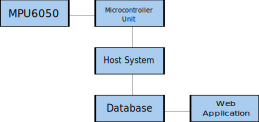
\includegraphics[scale=0.2]{flowchart.pdf}
            \caption{Depicting Collected Data of Gy}
            \label{fig:archi}
        \end{figure}
     \end{columns}
\end{frame}

%--------------------------------------------------------





%------------------------------------------------

\begin{frame}{Obtained Results}
    \begin{figure}
        \centering
        \includegraphics[scale=0.18]{Screenshot (292).png}
        \caption{Plotting Data and Depicting posture in Real-time.}
        \label{fig:results}
    \end{figure}
       
\end{frame}
%-----------------------------------------------



%------------------------------------------------
\section{Conclusions and Future Work.}
%------------------------------------------------

\begin{frame}{Limitations and Future Work}
    \begin{block}{Limitations}
        \begin{itemize}
            \item Can be susceptible to noisy movements.
            \item Be able to detect more range of activities.
        \end{itemize}
    \end{block}
    \begin{block}{Future Work}
        \begin{itemize}
            \item Send http requests without the intervention of host system.
            \item Give a detailed analysis of their posture and predict it's effect on health.
        \end{itemize}
           
    \end{block}
    
\end{frame}

%------------------------------------------------




%-----------------------------------------------
\begin{frame}
    
         \Huge{\centerline{Thank you.}
         \vspace{1cm}
         \Huge{\centerline{Questions}
         }
         }
    
\end{frame}



%----------------------------------------------------------------------------------------

\end{document}
